% !TEX root = ../../main.tex
% !TeX spellcheck = de_DE

\chapter{Stand der Technik}

\section{General Adversarial Network}

Der Begriff GAN \textit{(General Adversarial Network)} ist auf Ian Goodfellow zurückzuführen \cite{gan-original-paper}.
Das Wort bezeichnet ein Konstrukt aus 2 neuronalen Netzen, die sich gegenseitig trainieren.
Durch das spezielle Training gelingt die Generierung von unechten aber realistischen Daten.
Solche Daten können dann zum Beispiel für das Training anderer neuronalen Netze \cite{gan-application-augmenting-training-data}, Bildbearbeitung \cite{gan-application-upscaling, gan-application-blending} und vielen mehr verwendet werden \cite{gan-application-dna-optimizes-protein-functions, gan-application-audio-synthesis}.
\newline

Die beiden Netze eines GANs werden in den Generator und den Discriminator unterschieden.
Aufgabe des Generators ist die Generierung von unechten Daten.
Dafür wandelt er eine zufälligen Eingabe in einen möglichst realistischen Output um.
Die zufällige Eingabe dient dabei als Basis für die Ausgabedaten.
Das ist notwendig, da der Umwandlungsprozess selbst deterministisch ist, aber trotzdem eine Vielzahl an unterschiedlichen Daten generiert werden soll.

Der Output des Generators wird dann vom Discriminator klassifiziert.
Dafür wird er sowohl auf die generierten Daten als auch einen Bestand an echten Daten trainiert.
Sein Ziel ist es dann, die falschen Daten des Generators zu identifizieren.
Ziel des Generators hingegen ist es, dass sich der Discriminator irrt und die generierten Daten als echt einstuft.

Ian Goodfellow bezeichnet den Lernprozess auch als Minimax-Spiel, bei die Ausgabe des Discriminators die zu optimierende Größe ist.
Das heißt, der Generator versucht diese zu verkleinern, während der Discriminator sie erhöhen möchte. \cite{gan-minimax} 

\begin{figure}[H]
	\centering
	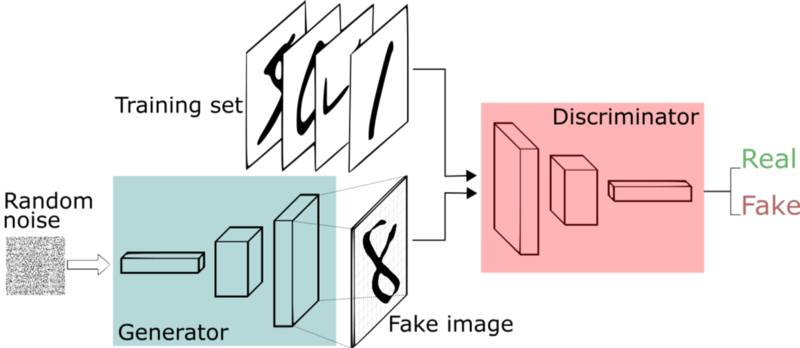
\includegraphics[width=12cm]{kapitel/2_stand_der_technik/img/GAN.png}
	\label{img:gan}
	\caption{Generative Adversarial Network (Bild von Thalles Silva \cite{img-gan})}
\end{figure}

Für diese Arbeit werden zusätzlich Label eingeführt, um die generierten Daten beeinflussen zu können. 
Diese Art von GAN nennt sich CGAN oder Conditional GAN \cite{gan-conditional}.
Dazu erhalten der Generator und Discriminator das Datenlabel als einen weiteren Input.
So kann der Discriminator aus den echten Daten lernen, dass Daten bei bestimmten Labeln bestimmte Eigenschaften haben.
Dadurch ist dann der Generator gezwungen, diese Eigenschaften zu berücksichtigen, um den Discriminator wieder zu täuschen.

\section{Hyperparameter}
Hyperparameter sind Invarianten, die den Lernprozess beeinflussen.
Es handelt sich um Invarianten, da sie beim Training im Gegensatz zu Parametern unveränderlich bleiben.
Hyperparameter sind sehr wichtig, das sie einen starken Einfluss auf den Trainingsprozess haben (\cref{chapter:hyperparameter-einfluss}).
Beispiele für Hyperparameter wären zum Beispiel Lernrate oder Dropout (\cref{chapter:hyperparameter-arten}).

\subsection{Einfluss von Hyperparametern}
\label{chapter:hyperparameter-einfluss}
Hyperparameter werden genutzt, um neuronale Netze statisch zu konfigurieren.
Im Gegensatz zu den Parametern, die im Trainingsprozess gelernt werden, ändern sie sich nicht.
Bei den Hyperparametern handelt es sich zum Beispiel um die Lernrate, Anzahl an Neuronen in bestimmten Schichten, Lossfunktion und viele andere \cite{hyperparameters-gan-using-genetic-algorithm}.
\newline

Das setzen der Hyperparameter ist essentiell für den Trainingserfolg, weshalb es diverse Studien zur Bestimmung optimaler Hyperparameter gibt \cite{hyperparameters-gan-using-genetic-algorithm, hyperparameters-using-genetic-algorithm-2, hyperparameters-grid-search}. \todo{Quellen verwenden, die nicht noch einmal benutzt werden}
Aber nicht jeder Hyperparameter hat einen gleich großen Auswirkung auf den Trainingserfolg \cite{hyperparameters-search-in-machine-learning}.
Ein Beispiel für einen sehr einflussreichen Hyperparameter wäre zum Beispiel die Lernrate, deren Optimierung immer zumindest in Betracht gezogen werden sollte \cite{learning-rate-most-important}.
\newline

\todo{keine Belege gefunden - stimmt das?}
Zusätzlich ist zu erwähnen, dass Hyperparameter nicht nur das Training beeinflussen sondern auch andere Hyperparameter. 
So können manche Parameter in bestimmten Kombinationen stark an Einfluss gewinnen, während andere unwichtiger werden.
Das ist insbesondere bei den Verfahren zur Bestimmung der Hyperparameter ein Problem.
Denn dadurch muss immer eine Kombination getestet und verglichen werden, was deutlich rechenaufwändiger ist, als die Parameter einzeln zu testen.


\subsection{Verfahren zur Bestimmung von Hyperparametern}
\url{https://towardsdatascience.com/understanding-hyperparameters-and-its-optimisation-techniques-f0debba07568}
Die Optimierung von Hyperparametern ist ein bekanntes Problem bei dem bereits mehrere Lösungsverfahren entwickelt wurden.
Einige Verfahren werden im Folgenden näher erläutert.

\paragraphNewLine{Manuelle Suche}
Zunächst ist es möglich die Hyperparameter manuell festzulegen 
Zwar wird so sehr viel Rechenaufwand eingespart, da nur eine oder sehr wenige Konfigurationen getestet werden.
Das System ist jedoch sehr aufwändig für die Person, die es konfiguriert.
Zum einen müssen die Werte manuell geändert werden, zum anderen muss eine sehr bedachte Vorauswahl getroffen werden.
Zusätzlich müssen die Ergebnisse auch manuell analysiert werden, um Patterns zu erkennen und so neue Durchläufe zu planen.

\paragraphNewLine{Gridsearch - Rastersuche}
Bei der Rastersuche handelt es sich um eine sehr traditionelle Technik und ist gut mit einem Brute-Force Ansatz vergleichbar \cite{hyperparameters-grid-search}.
Zunächst wird werden die zu untersuchenden Hyperparameter ausgewählt.
Danach erfolgt die Definition eines Suchintervalls inklusive Intervallschritten für jeden Hyperparameter.
Schließlich wird das neuronale Netzwerk für jede Kombination trainiert und die Ergebnisse der einzelnen Durchläufe festgehalten.
\newline

Im nächsten Schritt ist es dann möglich, die einzelnen Ergebnisse zu vergleichen.
Dabei können dann Schemata erkannt und Kombinationen aussortiert werden.
Es ist dann möglich die erfolgversprechendsten Netze weiter zu trainieren, oder direkt eine zufriedenstellende Kombination auszuwählen.
\newline

Insgesamt ist Gridsearch sehr simpel zu implementieren, aber auch sehr ressourcenaufwändig.
Der exakte Aufwand hängt dabei stark von der Anzahl der möglichen Kombinationen der Hyperparameterwerte ab.
Weil es sich bei den Kombinationen um ein ein Kreuzprodukt handelt, wächst der Aufwand mit der Anzahl an Werten auch sehr stark an.
Durch die Möglichkeit von Parallelisierung findet die Gridsearch in der Regel bessere Parameter als die sequentielle manuelle Suche in der gleichen Zeit \cite{hyperparameters-random-search}.

\paragraphNewLine{Random Search}
Die Random Search \cite{hyperparameters-random-search} funktioniert ähnlich wie die Gridsearch, nur werden zufällige Werte statt einem festgelegten Werteraster erzeugt (\cref{img:random-search}).
Die zufälligen Werte haben den Vorteil, dass es weniger Werte-Überlagerungen im Vergleich zur den Raster-Kombinationen gibt.
Deswegen kann die zufällige Suche bei gleich vielen Durchläufen ein größeres Spektrum an Ergebnissen abdecken.
Mittels \textit{Automatic Relevance Determination} \cite{automatic-relevance-determination} ist es dann möglich, den Einfluss und Wertebereich der einzelnen Hyperparameter darzustellen.

\begin{figure}[H]
	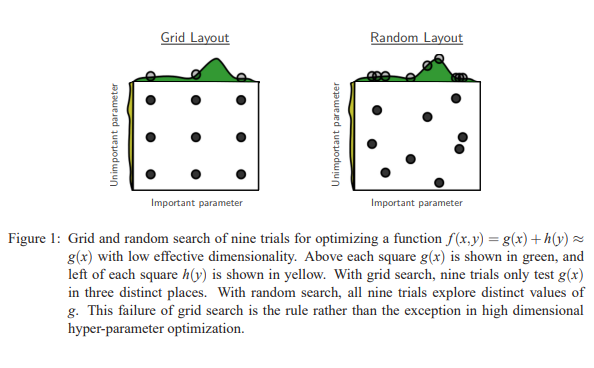
\includegraphics{kapitel/2_stand_der_technik/img/random-vs-grid-search.png}
	\caption{Random Search vs Grid Search (Quelle \cite{hyperparameters-random-search})}
	\label{img:random-search}
\end{figure}

Problem der Random Search ist vor allem, dass die Räume der guten Hyperparameter (\textit{Search Space}) sehr klein sind.
Dadurch ist nicht gewährleistet, dass ein zufälliger Wert auch den Raum trifft.
Jedoch erzielen Optimierungen mittels Random Search in der Regel trotzdem (sehr) gute Ergebnisse.
Dem Grid-Search-Verfahren ist die Random-Search allerdings nicht prinzipiell überlegen \cite{hyperparameters-random-search}.

\paragraphNewLine{Genetic Algorithm - Evolutionäre Suche}
\todo[inline,shadow]{mehr belegen}
Das evolutionäre Suchverfahren wandelt die Hyperparametersuche in einen evolutinären Entwicklungsprozess um.
Die 'Evolution' des Algorithmus ist eine Anlehnung an die natürliche Entwicklung in der Natur.
Diese Entwicklung zeichnet sich durch die Operatoren Selektion, Kombination und Mutation aus, die auch der Algorithmus verwendet. \cite{hyperparameters-search-comparison-focus-genetic, hyperparameters-genetic-algorithm}
\newline

Für den Optimierungsprozess werden am Anfang mehrere zufällige Hyperparameterinstanzen erzeugt.
Die Instanzen werden dann trainiert und stehen im Wettbewerb um das beste Ergebnis.
Nach der Auswertung der Trainingsergebnisse werden die besten Instanzen selektiert und miteinander gekreuzt und oder mutiert.
\newline

Die evolutionäre Suche eignet sich besonders gut bei sehr vielen Hyperparametern.
Im Gegensatz zur Grid-Search werden nicht immer alle Kombinationen ausprobiert, sondern nur einzelne, die sich bereits zuvor als vielversprechend herausgestellt haben.
Dadurch kann mit sehr großen Mengen an Hyperparametern umgegangen werden.

Allerdings ist die evolutionäre Suche vergleichsweise langsam, da die Evolutionsschritte sequentiell ablaufen müssen.
Erst bei einer hohen Anzahl an Hyperparametern oder einem sehr großen Suchraum wird die Grid-Search dann so langsam, dass sich die evolutionäre Suche lohnt \cite{hyperparameters-search-comparison-focus-genetic}.


\paragraphNewLine{Bayessearch}
\todo[inline,shadow]{noch beschreiben, irgendwie kompliziert...}
\begin{itemize}
	\item Ziel: Anzahl der Versuche reduzieren
	\item Idee: Wiederverwendung von vorherigen Durchläufen
	\item ??
\end{itemize}

\subsection{Auswahl bestimmter Hyperparameter}
\label{chapter:hyperparameter-arten}
Zwar haben Hyperparameter insgesamt einen großen Einfluss auf das Training, jedoch nicht jeder einzelne gleich viel (\cref{chapter:hyperparameter-einfluss}).
Deshalb werden in dieser Arbeit auch nur eine Auswahl an Parametern analysiert, die in der Regel einen großen Einfluss auf das Ergebnis haben. \todo{Quelle oder andere Begründung}
Die zu analysierenden Parameter werden im Folgenden genauer beschrieben.

\paragraphNewLine{Lossfunction}
Die Lossfunction wird genutzt, um den Lernfortschritt von neuronalen Netzen zu bestimmen.
Dafür wird der Unterschied zwischen dem Erwartungswert und dem Ergebnis berechnet.
Einfache Beispiele sind der \textit{Absolute Value Loss} und \textit{Squared Error Loss}:
\begin{itemize}
	\item Absolute Value Loss: $L_1(y, \hat{y}) = |y - \hat{y}|$
	\item Squared Error Loss: $L_2(y, \hat{y}) = (y - \hat{y})^2$
\end{itemize}

Bei der Interpretation des Wertes gibt es jedoch einige Aspekte zu beachten.

Zum einen gibt es \textit{Noise}, der die Verfälschung eines Datensatzes im Vergleich zum Optimum angibt.
Das ist zum Beispiel der Fall, wenn im Bild ein Rauschen existiert.
Durch das Rauschen kann dann der Erwartungswert nicht mehr exakt bestimmt werden, da das Ergebnis nicht mehr zu 100\% feststeht.

Dann kann es sein, dass das Trainingsset zu klein ist.
So ist eventuell das Optimum gar nicht durch die Trainingsdaten ableitbar.
In diesem Fall müssen zwar die Daten angepasst werden, aber die Lossfunktion sollte eine solche Approximation in Betracht \todo{bitte was?} ziehen. 

Zuletzt kann auch das Gegenteil der Fall sein, dass zu viele Daten existieren und gar nicht alle zum Training verwendet werden.
Auch dann muss das Optimum wieder approximiert werden.

Insgesamt sollte die Lossfunction also nur als Fehler für ein Datum und nicht den Datensatz angenommen werden.
Um den Loss für alle Daten zu errechnen, lohnt es sich einen Batch zu nehmen und diesen dann für den Datensatz zu interpolieren.

\paragraphNewLine{Learning Rate}
Um den Fehler aus der Lossfunction auch zum Lernen zu verwenden wird eine zusätzlich die Lernrate eingeführt.
Diese ist notwendig, was durch den Fall $Lernrate = 1$ veranschaulicht werden kann.

Aufgrund der gewählten $Lernrate = 1$ würde das Netz auf jeden Datensatz trainiert werden, als ob es der optimale Fall ist.
Problem daran ist, dass so nicht das Abstrahieren erlernt wird.
Das neuronale Netzwerk wird am Ende ein Datum (und zwar das zuletzt trainierte) genau erkennen können.
Alle anderen Daten werden dann höchstens aufgrund ihrer Ähnlichkeit zum optimalen Datum erkannt.
\newline

Aus diesem Grund wird eine Lernrate eingeführt, die den Lernprozess auf mehrere Datensätze aufteilt.
Dadurch kann das neuronale Netzwerk dann theoretisch Korrelationen zwischen Daten erkennen und diese lernen.
Als guter Standartwert wird oft $10^(-5)$ empfohlen. \todo{Quelle -> Zahl anpassen oder rausnehmen}
\newline

Da sowohl die Lernrate als auch die Lossfunction für den Lernprozess verwendet werden, ergibt sich dadurch unweigerlich ein Zusammenhang zwischen den Größen.
\todo{Recherche - Abhängigkeit zwischen Lernrate und Lossfunction}
\todo{wieder Bogen schließen zum Anfang, wo die Zusammenhänge zwichen den Parametern erklärt werden}
\newline

Durch die Lernrate kann vor allem die Lerngeschwindigkeit beeinflusst werden.
Die sollte am Anfang relativ hoch sein und gegen Ende zur Feinjustierung abnehmen.
\todo{deutlich mehr dazu schreiben}

Außerdem wird in zwei Prinzipien für Lernraten unterschieden.
Entweder exisitert eine Lernrate um das gesamte Netz zu trainieren, oder eine eigenständige Lernrate für jedes Neuron.
Der zweite Fall ist zwar wieder aufwändiger, aber dafür kann so Gradientdescent verhindert werden.
\todo{stimmt das? wo werden diese typischen Probleme gradientdescent,... von neuronalen netzen und auch speziell gans besprochen?}

Manche Quellen bezeichnen die Lernrate als wichtigsten Hyperparameter, der immer angepasst werden sollte \cite{learning-rate-most-important}

\paragraphNewLine{Number of Units}
Mit den Number of Units ist die Anzahl der Neuronen gemeint.
Die Anzahl beeinflusst direkt die maximale Lernfähigkeit des Neuronalen Netzwerks.
Denn je mehr Neuronen, desto mehr Parameter können gelernt werden und folglich feiner auf die Trainingsdaten abgestimmt werden.
\newline

Mehr Parameter für das Neuronale Netzwerk bedeutet aber auch ein höherer Lernaufwand.
Deshalb ist es nicht ratsam, die Parameteranzahl beliebig zu erhöhen.
Falls ein sehr großes Netz benötigt wird, existiert auch die Möglichkeit des Transferlearnings. 
Hierfür wird ein Netzwerk auf Daten vortrainiert.
Danach kann es dann für andere Datensätze verwendet werden und muss nur noch minimal nachtrainiert werden. \todo{Quelle, sinnvoll zu erwähnen?}
\newline

Bei der GAN-Architektur \todo{gan architektur vorher richtig beschreiben} eignet sich eine variable Anzahl an Neuronen vor allem in den letzten Layern des Discriminators.
Dabei handelt es sich normalerweise um Dense-Layer. \todo{normalerweise -> durch unsere ersetzen?}
Die theoretische Aufgabe der Dense-Layer ist dabei die Informationen aus den vorherigen Convolutional Layern zu extrahieren.
Somit hat diese Schicht einen verhältnismäßig großen Einfluss auf den Erfolg des Discriminators und somit auch auf das GAN.


\section{Related Work}
Es gibt viele verschiedene Versuche und Varianten die Hyperparameter zu optimieren.
Dementsprechend viele Papers und Artikel befassen sich damit.
Einige dieser Arbeiten werden nachfolgend kurz vorgestellt.
\newline

\paragraphNewLine{Best Selection of Generative Adversarial Networks Hyper-Parameters Using Genetic Algorithm \cite{hyperparameters-genetic-algorithm}}
Die Studie befasst sich mit Hyperparameter Optimierung auf Basis von genetischen Algorithmen.
Genetische Algorithmen zeichnen sich unter anderem durch die verwendeten Operatoren Mutation, Kreuzung und Selektion aus \cite{genetic-algorithms}.
Ziel der Studie war es, bestmögliche Hyperparameter für das MNIST Datenset zu finden \cite{dataset:mnist}.
Dabei wurden die Hyperparameter \textit{learning-rate, dropout, batch-size und number of neurons in dense layer} betrachtet.
Ergebnis war eine 100\% Genauigkeit im Vergleich zu 96\% des Vergleichsnetzes.
\newline

Zwar sind die Daten und die Herangehensweise nicht die selbe wie in dieser Arbeit, aber die untersuchten Hyperparameter.
Diese können mit als Basis für die Untersuchung genommen werden.
Zudem verdeutlicht die Arbeit noch einmal die große Auswirkung von Hyperparametern.

\paragraphNewLine{Unsupervised Representation Learning With Deep Convolutional Generative Adversarial Networks \cite{hyperparameters-convolutional-gan}}
Ziel dieser Studie ist es allgemein gute Hyperparameter zu finden.
Dafür wurden Bilder aus verschiedenen Datensets genommen (Large Scale Scene Understanding \cite{dataset:lsun}, Imagenet-1k \cite{dataset:image-net} und einem eigenen Datenset mit Gesichtern).
Bei den Hyperparametern wurden diverse untersucht, zum Beispiel aber nicht ausschließlich die Lernrate, Momentum und Batch-Size.
Im Ergebnis konnten für alle Werte gefunden werden, die über alle Datensets meistens stabil mit zufriedenstellenden Ergebnissen liefen.
\todo{Hyperparameter: learning-rate 0.0002, momentum (beta1) zu 0.5, mini-batch size 128,... (Kapitel 4 Details of adversarial training)}
Erkenntnis der Studie war auch, dass keine Hyperparameter Kombination gefunden werden konnte, die über alle Datensets 100\% stabil laufen konnte.
\newline

Eine allgemeine Studie zum Thema Hyperparameter ist für die Arbeit sehr interessant, da sie gute Ausgangswerte bietet.
Dass keine 100\% stabile Zusammenstellung gefunden werden konnte, verdeutlicht die Notwendigkeit der Feinanpassung an jedes Datenset.


\paragraphNewLine{The GAN Landscape: Losses, Architectures, Regularization, And Normalization \cite{gan-landscape-losses-architectures-regularization-normalization}}
Dieses Studie beschäftigt sich nicht ausschließlich mit Hyperparametertuning.
Aber auch in dieser Studie werden allgemein GANs optimiert und die Erkenntnisse daraus können verwendet werden.
In the GAN Landscape wird das GAN auf die Datensets CIFAR10 \cite{dataset:cifar10}, CELEBA-HQ-128 und LSUN-BEDROOM \cite{dataset:lsun}.
Für das Training wurden dann ein DCGAN und ResNet verglichen.
Dabei fand die Studie viele interssante Erkenntnisse heraus, zum Beispiel eine gute Updatequote von 5:1 zwischen Discriminator und Generator.
\newline

Besonders interessant bei dieser Arbeit ist die Bestimmung von anderen Methoden, wie das unterschiedliche Updaten von Discrimintaor und Generator.
Wieder bietet die Arbeit eine gute Ausgangslage, aber keine Lösung für ein Datenset mit geometrischen Bildern.

\paragraphNewLine{Tunability: Importance of Hyperparameters of Machine Learning Algorithms}
\url{https://www.jmlr.org/papers/volume20/18-444/18-444.pdf}

\begin{comment}
	
\paragraph{Links}
\begin{itemize}
	\item Inception Score zum Rating von erzeugten Bildern (Salimans et al. 2016)
	\item Frechet Inception Distance (Heusel et al. 2017)
	\item stackoverflow \url{https://stackoverflow.com/questions/46386948/adjusting-gan-hyperparameters}
	\item \url{https://openreview.net/pdf?id=rkGG6s0qKQ}
	\item \url{https://arxiv.org/pdf/1511.06434.pdf%C3%AF%C2%BC%E2%80%B0}
	\item Forget the Learning Rate, Decay Loss \url{https://arxiv.org/ftp/arxiv/papers/1905/1905.00094.pdf}
	\item beste learningRate/Dropout/BatchSize/NumberOfNeuronsInDenseLayer mit evolutionären neuronalen netz für mnist 
	\item zum orientieren ?? \cite{gan-conditional}
\end{itemize}


\end{comment}